\providecommand{\mainpath}{..} % Command to retrieve the path of the main file. It must be defined before documentclass.

\documentclass[\mainpath/main]{subfiles}
\begin{document}

\chapter{Project Estimations} % First chapter
\label{ProjectEstimation}

% Command to be executed after the starting of every chapter
\setmyfancystyle
% ----------------

In this chapter we are going to estimate the main features of \textit{myTaxiService} project, by using COCOMO II. Reading from the reference manual:
\begin{quote}
	\textit{The COCOMO II model is part of a suite of Constructive Cost Models. This suite is an effort to update and extend the well-known COCOMO (Constructive Cost Model) software cost estimation model originally published in Software Engineering Economics by Barry Boehm in 1981.}
\end{quote}
In the \autoref{ProjectEstimation:ProjectSize} we focus on the project's size in term of lines of code, whereas in the \autoref{ProjectEstimation:EffortEstimation} other metrics, such the required time and the costs will be analysed.



\section{Project Size (Function Points)}
\label{ProjectEstimation:ProjectSize}
Reading from the reference manual:
\begin{quote}
	\textit{The function point cost estimation approach is based on the amount of functionality in a software project and a set of individual project factors [Behrens 1983; Kunkler 1985; IFPUG 1994]. Function points are useful estimators since they are based on information that is available early in the project life-cycle. A brief summary of function points and their calculation in support of COCOMO II follows.}
\end{quote}
The function types are five, described in the table\footnote{The table is given by the COCOMO II reference manual.}.\\[0.2cm]
\begin{tabular}[!ht]{l@{\hspace{1cm}}p{8.5cm}}
	\hline  \textbf{Function Point} & \textbf{Description}\\ 
	\hline External Input (EI) & Count each unique user data or user control input type that enters the external boundary of the software system being measured.\\ 
	\hline External Output (EO) & Count each unique user data or control output type that leaves the external boundary of the software system being measured.\\ 
	\hline Internal Logical File (ILF) & Count each major logical group of user data or control information in the software system as a logical internal file type. Include each logical file (e.g., each logical group of data) that is generated, used, or maintained by the software system.\\
	\hline External Interface Files (EIF) & Files passed or shared between software systems should be counted as external interface file types within each system.\\
	\hline External Inquiry (EQ) & Count each unique input-output combination, where input causes and generates an immediate output, as an external inquiry type.\\ \hline \\[1cm]
\end{tabular}

Finally, to perform the analysis we have to present other two tables from the same reference manual of the other one. The first one will be used to classify each function on three level of complexity (high, medium and low).

\begin{figure} [!ht]
	\centering
	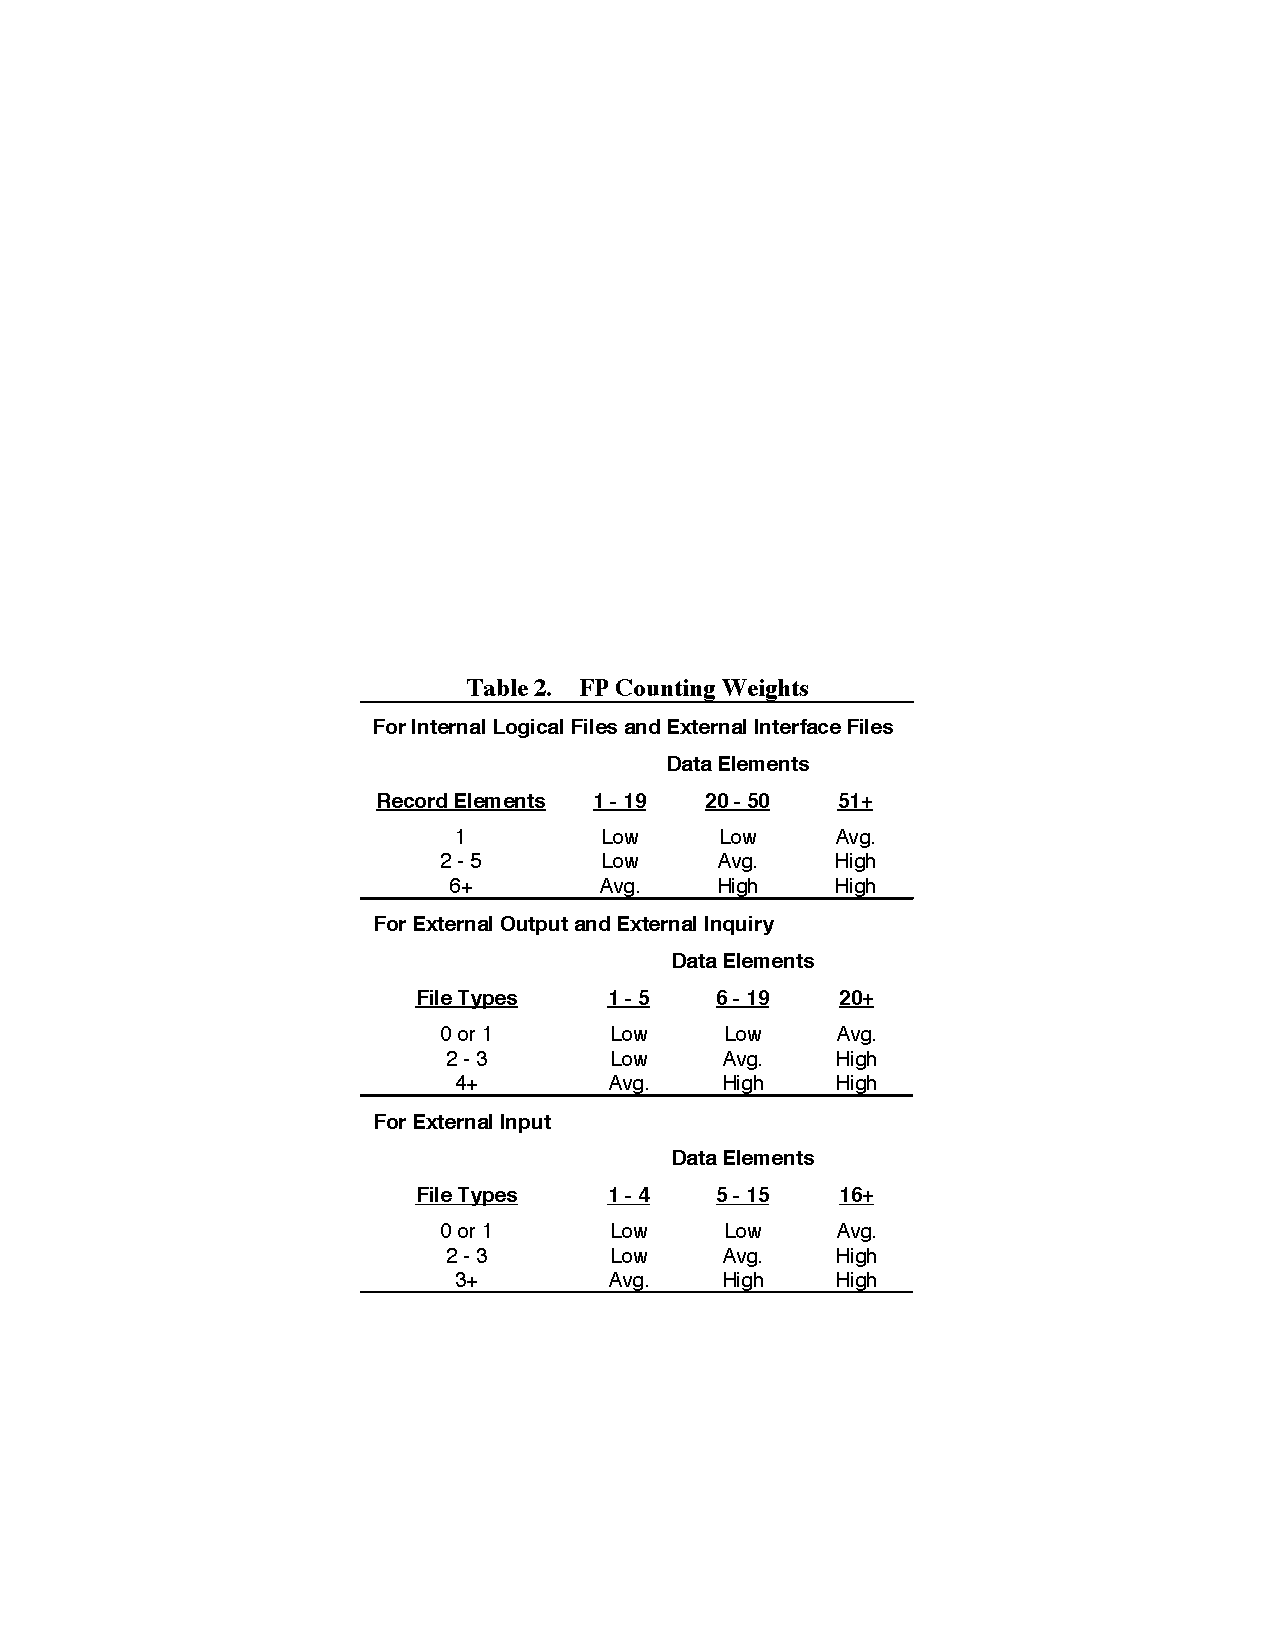
\includegraphics{table/complexity}
\end{figure}

The second one shows the weights to be used into the estimation formulas\footnote{The UFP acronym means Unadjusted Function Points}.

\begin{figure}[!ht]
	\centering
	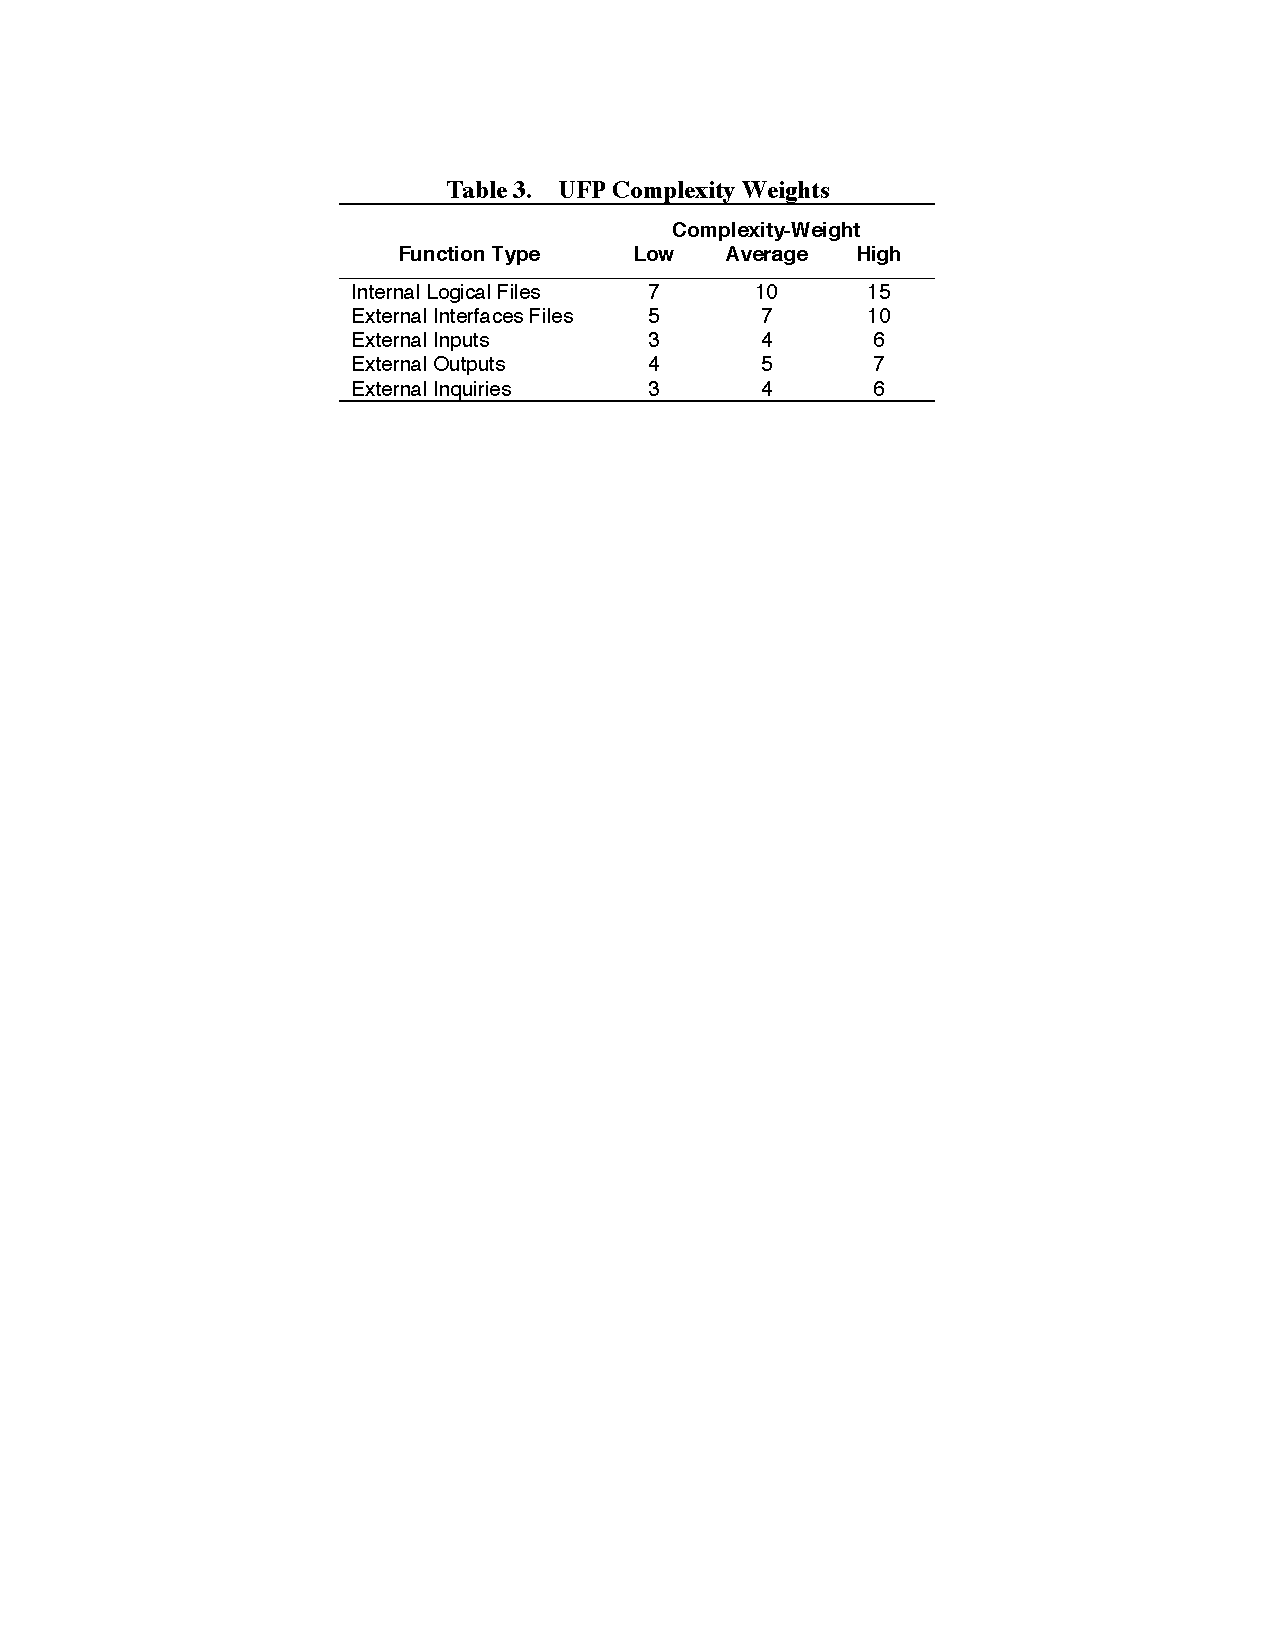
\includegraphics{table/weights}
\end{figure}

\clearpage

Up to now, we have presented the Function Points technique. Now, we are going to start our analysis, split by the function type.

\subsection{Internal Logic Files}
The system has to manage Internal Logic Files to store information related to the users (both \textit{normal} and drivers), the \textit{historical} rides, the areas and the driver workshifts\footnote{See the logic schema at the page 10 of the Design Document to have a detailed description of each part of the database.}\\
The users have from 12 to 16 fields to be stored (the second number is referred to the drivers case) and only the alerts and the zerotime or future rides have to be stored, thus the complexity is low. The areas and the workshifts can also be considered as low complexity type. In fact they have a few fields and less than six extra records.\\
The rides have 10 fields, including two positions, the driver and the passenger, all saved in separate entities. They can be considered as an average complexity type, since we have about seven records per ride (in fact in addition to the five presented, the positions requires additional records).\\
In the table the analysis is summarize:
\begin{tabular}{ccc}
	\hline ILF & Complexity & FP \\
	\hline User & Low & 7 \\
				Area & Low & 7 \\
				Workshift & Low & 7 \\
				Ride & Average & 10 \\
	\hline Total & & 31
\end{tabular}

\subsection{External Logic Files}
The system acquires data from te GPS interface. A GPS position is essentially a tuple of type Position, described in our database. Hence, we have a low complexity type and 7 FP.

\subsection{External Inputs}

\subsection{External Inquiries}

\subsection{External Outputs}


\section{Effort Estimation (COCOMO II)}
\label{ProjectEstimation:EffortEstimation}





\end{document}